\documentclass[a4paper,11pt]{article}
%Use article for short documents
\usepackage[T1]{fontenc}
\usepackage{parskip}
\usepackage{latexsym,amsmath,amssymb}
\usepackage{natbib}
\usepackage{graphicx}
\usepackage{times}
\usepackage{zi4}
\usepackage[a4paper,left=3cm,right=3cm,top=3cm,bottom=3cm]{geometry}

\title{The title}
\author{Your name}

\begin{document}
\maketitle
\thispagestyle{empty}
\newpage
\pagenumbering{arabic}

\section{Introduction}
My name is Susan Hutchinson. I work in the Department of Statistics and 
particularly enjoy teaching LaTeX. 

Some characters need to be typset carefully, for example \%, \# and \$.

\section{Research}

\subsection{A plot}
\begin{figure}[htb]
\centering
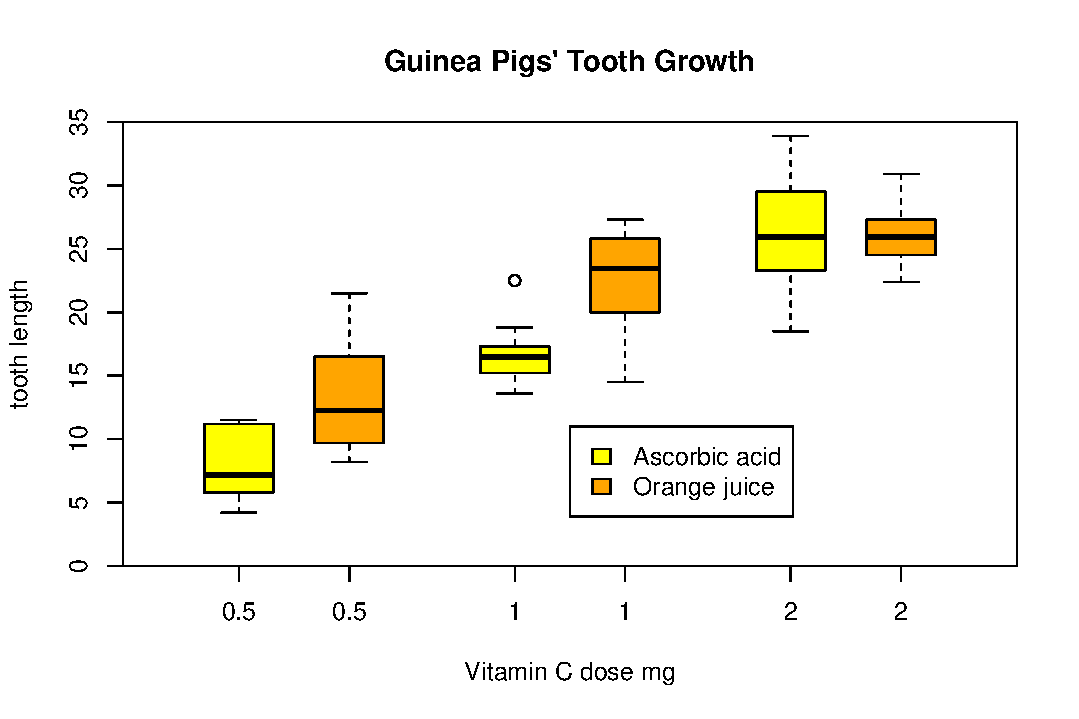
\includegraphics[width=4.8in, height=3.2in]{GuineaPigPlot.pdf}
\caption{Guinea pig tooth growth and vitamin C dose}
\label{fig:GPPlot}
\end{figure}

\subsection{Lists}
\begin{itemize}
\item Look before you leap
\item Then go for it
\item Enjoy the trip
\end{itemize}

This is a numbered list.
\begin{enumerate}
\item Frogs
\item Toads
\begin{enumerate}
\item Lesser spotted
\item Warty
\end{enumerate}
\end{enumerate}

\subsection{Maths}
This equation is part of the sentence: 
 $x\wedge (y\vee z) = (x\wedge y) \vee (x\wedge z)$ but the next one is
displayed separately.

$$\nabla^2 f(x,y) = \frac{\partial^2 f}{\partial x^2}
+ \frac{\partial^2 f}{\partial y^2}$$

\subsection{Tables}
A simple table

\begin{table}[htb]
\centering
\begin{tabular}{ll}
\textbf{Vegetables} & \textbf{Comments} \\
Carrots & Good early crop, then carrot fly. \\
French beans & Excellent.\\
\end{tabular}
\caption{Vegetable production}
\end{table}

\section{Conclusion}
Figure~\ref{fig:GPPlot} on page \pageref{fig:GPPlot} illustrates
the relationship between the amount of Vitamin C given and
their tooth growth \cite{Lamport}.

\clearpage
\section*{Appendix}
\begin{verbatim}
Put your R code here.
\end{verbatim}

\bibliographystyle{apalike2}

\bibliography{polygenic_bib}


\end{document}
